\documentclass[
  digital,     %% The `digital` option enables the default options for the
               %% digital version of a document. Replace with `printed`
               %% to enable the default options for the printed version
               %% of a document.
  oneside,     %% The `oneside` option enables one-sided typesetting,
               %% which is preferred if you are only going to submit a
               %% digital version of your thesis. Replace with `twoside`
               %% for double-sided typesetting if you are planning to
               %% also print your thesis. For double-sided typesetting,
               %% use at least 120 g/m² paper to prevent show-through.
  nosansbold,  %% The `nosansbold` option prevents the use of the
               %% sans-serif type face for bold text. Replace with
               %% `sansbold` to use sans-serif type face for bold text.
  nocolorbold, %% The `nocolorbold` option disables the usage of the
               %% blue color for bold text, instead using black. Replace
               %% with `colorbold` to use blue for bold text.         
  lof,         %% The `lof` option prints the List of Figures. Replace
               %% with `nolof` to hide the List of Figures.
  lot,         %% The `lot` option prints the List of Tables. Replace
               %% with `nolot` to hide the List of Tables.
  nocover
]{fithesis4}

\usepackage[resetfonts]{cmap}
\usepackage[T1]{fontenc}
\usepackage[main=english, slovak, czech]{babel}
\usepackage{paralist}
\usepackage{amsmath}
\usepackage{amsthm}
\usepackage{amsfonts}
\usepackage{url}
\usepackage{markdown}
\usepackage{rotating}

%% Enable inclusion of code samples with coloring
\usepackage{listings}
\usepackage{xcolor}
\definecolor{darkgreen}{rgb}{0.0, 0.6, 0.0}
\definecolor{darkred}{rgb}{0.6, 0.0, 0.0}
\definecolor{lightblue}{rgb}{0.17, 0.57, 0.69}
\definecolor{gray}{rgb}{0.5, 0.5, 0.5}

%% The following section sets up the metadata of the thesis.
\thesissetup{
    date        = \the\year/\the\month/\the\day,
    university  = mu,
    faculty     = fi,
    department  = ,
    type        = prop,
    author      = Mgr. Filip Petrovič,
    gender      = m,
    advisor     = {prof. RNDr. Luděk Matyska},
    title       = {Autotuning and optimization of compute kernels},
    TeXtitle    = {Autotuning and optimization of compute kernels},
    keywords    = {autotuning, GPU optimization, CUDA, OpenCL},
    TeXkeywords = {autotuning, GPU optimization, CUDA, OpenCL},
    universityLogo = fithesis-fi
}

\usepackage
[
    backend=biber,
    style=numeric,
    citestyle=numeric-comp,
    sorting=none,
    sortlocale=auto
    %% More information at <http://mirrors.ctan.org/macros/latex/contrib/biblatex/doc/biblatex.pdf>
]{biblatex}
\addbibresource{ThesisProposal.bib}

%% Index generation
\usepackage{makeidx}
\makeindex

\lstset
{
	frame=tb,
	language=C++,
	aboveskip=3mm,
	belowskip=3mm,
	showstringspaces=false,
	columns=flexible,
	basicstyle={\footnotesize\ttfamily},
	numbers=left,
	stepnumber=1,
	numberstyle=\tiny\color{gray},
	keywordstyle=\color{blue},
	commentstyle=\color{darkgreen},
	stringstyle=\color{darkred},
	breaklines=true,
	breakatwhitespace=true
}

\begin{document}

\chapter{Introduction}
In recent years, massively parallel devices such as modern CPUs and GPUs have become crucial in speeding up complex computations. These devices are used in areas such as physical simulations, weather forecasting, gaming, AI and many others. The speedup achieved by utilizing these devices can improve performance of these computations by several orders of magnitude. To employ these devices, a programmer needs to write the code in a specialized language such as OpenCL or CUDA. The programs written in these languages are called compute kernels.

However, there is a portability issue with these kernels because devices are manufactured by different vendors and their architectures have distinct properties and performance. This means the kernel code must be tailored for a specific device. This process is time consuming because it is done by expert programmers who must optimize the computation manually. The issue can be solved by autotuning \cite{balaprakash2018autotuning} which is an optimization method that involves code parametrization to create multiple versions of computation. Each of these parameters affects code performance in a specific way and the aim of autotuning is to find a well-performing combination of these parameters that are fit to the device being utilized.

The autotuning can be introduced either manually or by using a framework. The second option makes it significantly easier to integrate autotuning in real-world applications. These frameworks contain many features that would be difficult to implement manually. There are several different ones available to choose from. Kernel Tuning Toolkit is a framework developed at Faculty of Informatics, Masaryk University in Brno. The aim of this thesis is to research and introduce multiple new features into this framework to make the autotuning easier to use in practice.

\section{Thesis goals}
In this thesis, we focus on three main autotuning areas. They are the following ones:

\begin{itemize}
    \item Common autotuning format -- each of the autotuning frameworks has a specific programming API which is not portable. Certain APIs are not very well documented and can be quite complex to use. To solve this issue, we can create a high-level format to describe autotuned algorithms. Next, we want to develop an application which can convert this format into a framework-specific code. This will make it easier to port autotuned applications between different frameworks and make autotuning more accessible for programmers. Another benefit is that the format can be used in a benchmarking framework which compares performance of various autotuners and contains a shared database of autotuned code samples.
    \item Automatic tuning parameter generation -- currently, the tuning parameters need to be implemented by application developers, not by frameworks themselves. This can be rather difficult to achieve in more complex cases. It is possible to create a high-level language which generates certain common tuning parameters automatically. In this case, the tuning can be done transparently behind the scenes and programmer only needs to focus on writing application code. This can also make it easier for girls to write autotuning applications themselves. 
    \item Tuning space visualization -- it is difficult to imagine relations between different combinations of tuning parameters because the tuning output is only available in a text form. It is possible to create an application which would visualize these relations which would help developers to find certain hidden relationships between different parameters.
\end{itemize}

\chapter{Autotuning on parallel devices}

\section{Compute devices and APIs}
When we want to speed up a computation on parallel devices, we must write the code in a specialized language such as OpenCL or CUDA. Programs written in these languages are called compute kernels. OpenCL has an open API which is developed jointly by many companies and is supported on a wide range of devices (e.g., CPUs, GPUs, FPGAs, mobile devices). CUDA has a proprietary API developed by NVIDIA Corporation and it is focused mainly on GPUs made by NVIDIA. Both of these languages have similar programming model. An application is split into two parts -- a host application executed on a CPU and a kernel executed on a compute device. The host application is responsible for device management, memory management and kernel launching. The kernel usually contains the most computationally expensive part of application and that is why it executes many threads in parallel.

\subsection{Host application}
A host application is written in a regular language such as C or C++. It mostly handles inexpensive tasks such as data preparation, resource management and launching of compute kernels. OpenCL API defines the following structures which are needed to properly configure an OpenCL application:
\begin{itemize}
    \item \textit{Platform} -- An OpenCL platform represents an implementation of an OpenCL standard (e.g., a device driver developed by AMD, Intel or Nvidia).
    \item \textit{Device} -- Represents a specific compute device (e.g., AMD Ryzen 7 5800X, Nvidia GeForce RTX 3070). Devices are used for executing compute kernels.
    \item \textit{Context} -- A context holds all of the OpenCL runtime structures. It is akin to an operating system process. A context is created for a single OpenCL device and its lifetime is usually bound to an application runtime.
    \item \textit{Command queue} -- The commands such as launching of kernels and memory transfers are executed on an OpenCL device. These commands have to be submitted to a command queue where they are executed in a timely manner. It is possible to initialize multiple command queues within a single context to overlap independent operations.
    \item \textit{Buffer} -- Data accessed by a compute kernel have to be transferred into an OpenCL buffer. That is because kernels cannot directly acces the memory allocated by a host application. It is possible to specify a buffer memory location (device or host memory) and an access type (read and write access).
    \item \textit{Program} -- A program is compiled from an OpenCL C source file. Programs can be shared by multiple kernels so a single program has to be compiled only once.
    \item \textit{Kernel} -- Together, program and data create a compute kernel. The same compute kernel can be launched multiple times with different data.
    \item \textit{Event} -- Events serve as a synchronization primitive for individual commands submitted to a queue. It can also be used to retrieve information about a specific command such as computation status or duration.
\end{itemize}

An OpenCL application typically executes in the following phases:
\begin{enumerate}
    \item Platform and device selection
    \item Initialization of context and command queues
    \item Creation of memory buffers
    \item Program compilation and execution of a kernel function
    \item Transfer of data produced by a kernel from OpenCL buffers to host memory
\end{enumerate}

\subsection{Compute kernel}
Compute kernel is a function executed on a device. The kernel code is written from a perspective of a single \textit{work-item} which is the smallest OpenCL execution unit. Work-items operate in a lock-step mode so multiple work-items execute the same instruction on a different data in parallel. Each work-item has its own \textit{private memory} (i.e., the memory which is mapped to a CPU or a GPU register).

Work-items are organized into a larger structure which is \textit{work-group}. An OpenCL work-group can have up to three dimensions. The number and size of dimensions affects the amount of parallelism inside a kernel. The entire work-group is executed on a single \textit{compute unit} (e.g., a CPU core, a GPU streaming multiprocessor). It is possible for multiple work-groups to be executed on the same compute unit. On a work-group level, the work-items can access \textit{local memory} which is shared by all items belonging into the same group.

Work-groups are organized into an \textit{NDRange} (N-Dimensional Range). The size of NDRange depends on the size of input data that needs to be processed by a kernel. At this level, it is possible to utilize two types of memory -- \textit{global memory} and \textit{constant memory}. Global memory (e.g., CPU main memory, GPU global memory) is usually very large but has high latency. On the other hand, constant memory has smaller capacity but lower latency. It can be utilized to store read-only data. Certain devices such as CPUs do not have hardware support for constant memory and usually store such data in global memory. The entire OpenCL work-item and memory hierarchy is illustrated in Figure \ref{opencl-hierarchy}.

\begin{figure}
    \begin{center}
    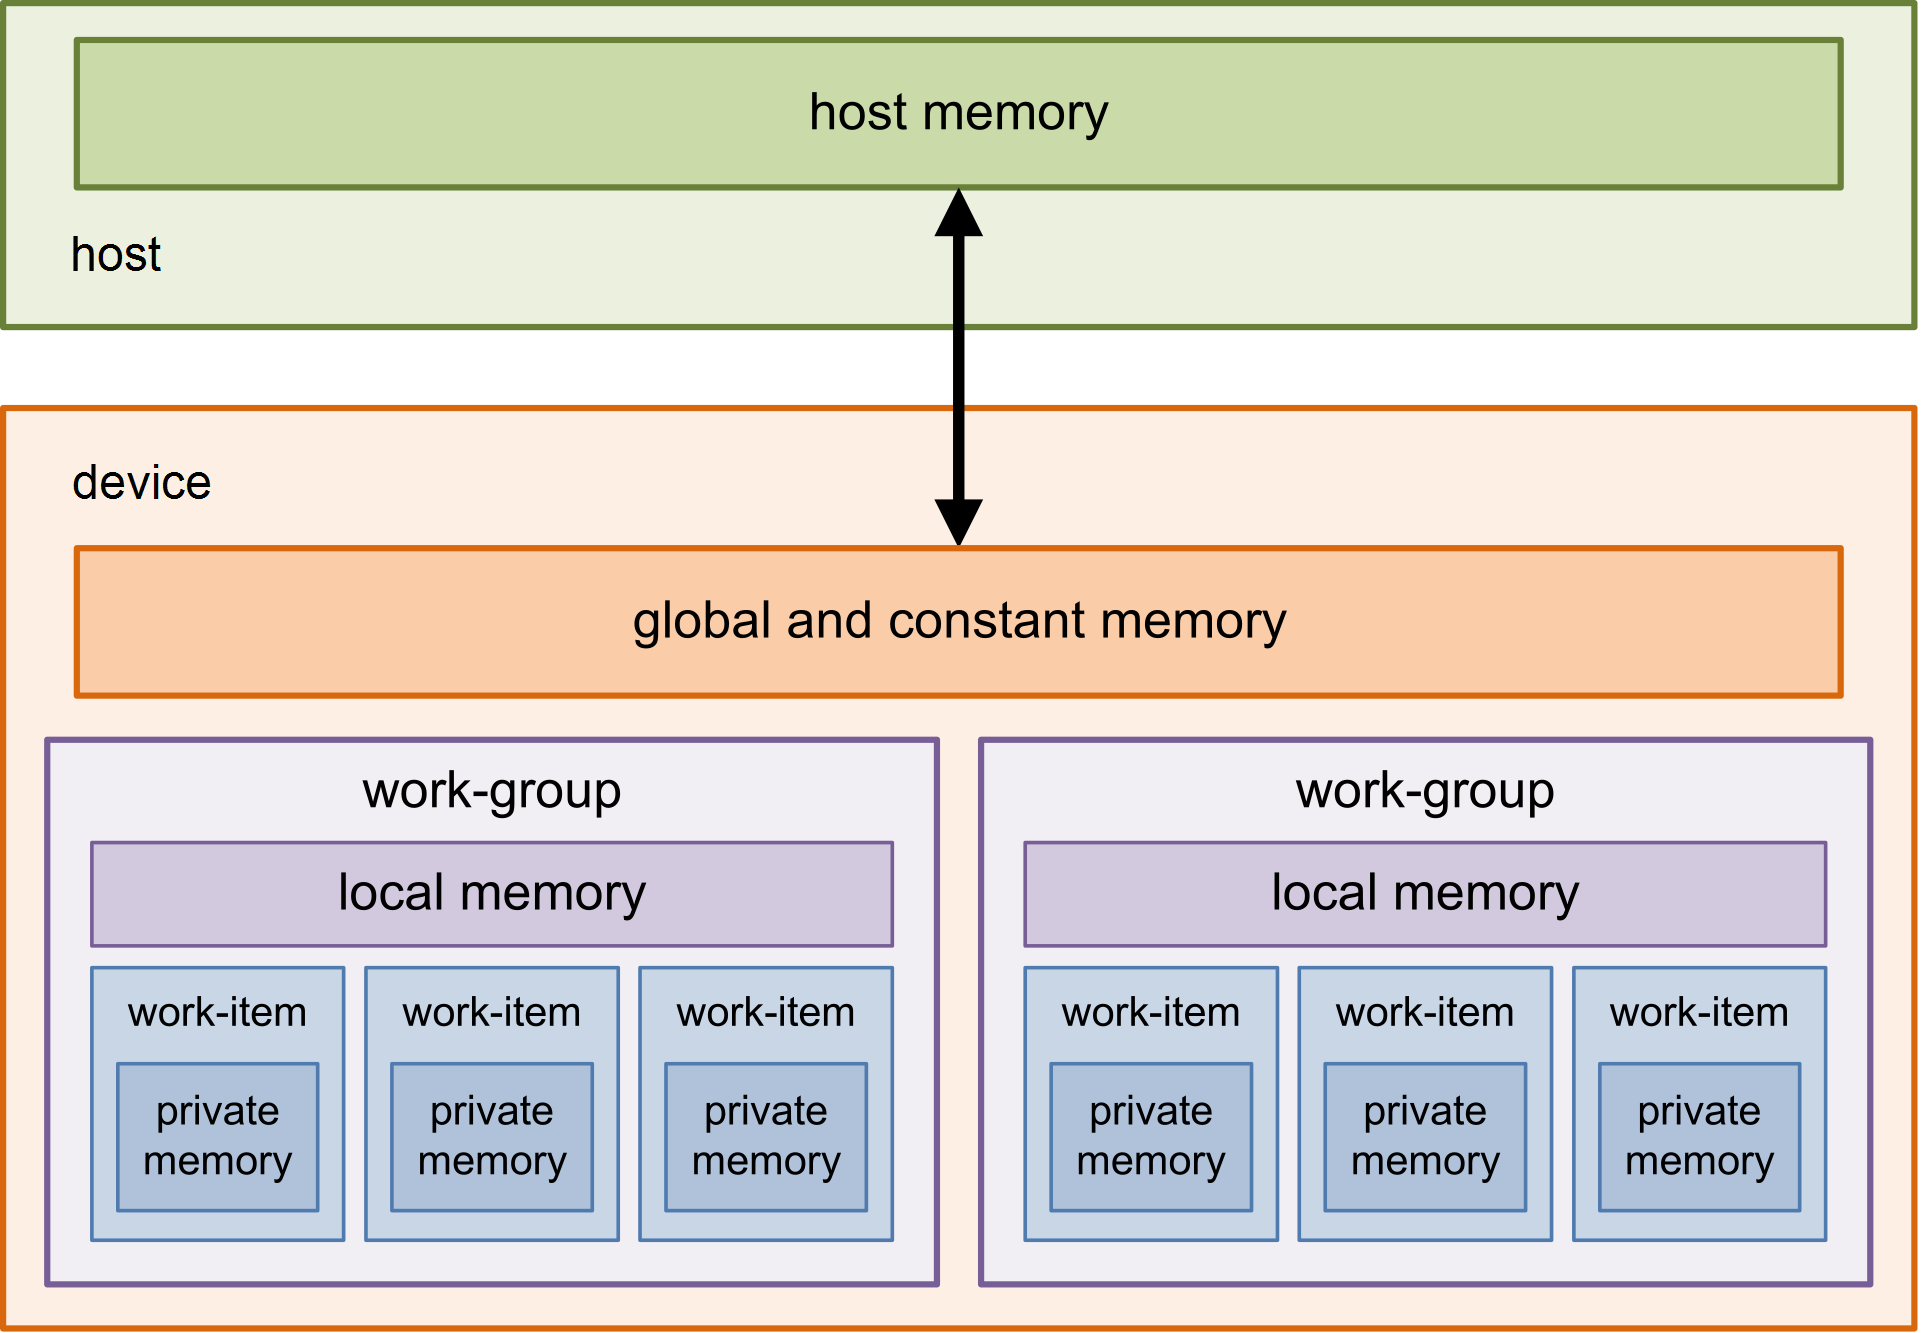
\includegraphics[width=125mm]{Figures/OpenClHierarchy.png}
    \end{center}
    \caption{OpenCL work-item and memory hierarchy, source: \cite{opencl-hierarchy-diagram}.}
    \label{opencl-hierarchy}
\end{figure}

\subsection{Compute kernel example}
A simple kernel function which performs a vector addition is shown in Figure \ref{vector_addition}. The kernel performs an addition of elements from arrays \textit{a} and \textit{b}, and then stores the result in array \textit{c}. The qualifier \textit{\_\_global} is used to mark kernel arguments which are stored in global memory. The function \textit{get\_global\_id(int)} retrieves a unique work-item index in the specified dimension. This index maps each work-item to a different array element.

\begin{figure}
\begin{lstlisting}
__kernel void vectorAddition(__global float* a, __global float* b, __global float* c)
{
    int i = get_global_id(0);
    c[i] = a[i] + b[i];
}
\end{lstlisting}
\caption{Vector addition kernel in OpenCL C language.}
\label{vector_addition}
\end{figure}

\subsection{Differences between OpenCL and CUDA}
CUDA language is very similar to OpenCL in available features and functionality. However, there are some differences that play a significant role during development of autotuned applications:
\begin{itemize}
	\item CUDA is officially available only for graphics cards released by NVIDIA Corporation. Devices developed by other vendors are not supported. \footnote{PGI compiler provides CUDA support for CPUs but is now deprecated.}.
	\item Global indexing (i.e., NDRange in OpenCL, grid in CUDA) works differently. In OpenCL, an NDRange size is specified as a size of work-group multiplied by a number of work-groups. However, grid size in CUDA is specified only as a number of blocks (CUDA term for work-groups). This is rather inconvenient for porting autotuned programs between CUDA and OpenCL. That is because some tuning parameters can affect the size of NDRange (grid).
	\item CUDA kernels have support for templated types which make it easier to implement some autotuning features.
	\item Identical or similar features may have different names (e.g., work-items are called threads in CUDA).
\end{itemize}

\section{Autotuning}
This chapter describes common terms used in relation to auto-tuning and provides a list of desired features which should be supported by autotuning frameworks. Afterwards, several generic frameworks are presented, including their advantages, disadvantages, usage examples and comparison. Frameworks which are domain-specific or not publicly available are not discussed here.

\subsection{Auto-tuning glossary}
The following terms are commonly encountered in subsequent chapters and their knowledge is required for better understanding of auto-tuning process:
\begin{itemize}
	\item \textit{tuning parameter} -- Parameter which, depending on its value, affects performance of a computation. For example, a parameter which controls length of a vector type of some variable. The exact way parameter comes into effect depends on a specific framework. Common option is a utilization of just-in-time compilation and preprocessor macros.
	\item \textit{configuration space} -- Space which is created as a Cartesian product of all tuning parameters and their values. Certain elements of configuration space may be eliminated by utilizing constraints.
	\item \textit{tuning configuration} -- Single element of configuration space.
	\item \textit{traversal of configuration space} -- A process where tuned program is launched repeatedly with different tuning configurations and its running time is measured.
	\item \textit{search method} -- A method employed to explore individual tuning configurations. Because configuration space may become very large,	exhaustive search is not always a viable option. It is possible to explore the space randomly or utilize an optimization method.
\end{itemize}

\subsection{Features of auto-tuning frameworks}
While there are no strict requirements over functionality that should be available in auto-tuning frameworks, there are several features which are either commonly implemented by existing frameworks or desired by users. They include the following: 
\begin{itemize}
	\item Scope of tuning parameters -- While definition of tuning parameters is supported by essentially all frameworks, not all of them allow parameters to affect all parts of a program. For example, some frameworks support only parameters which affect kernel code but not host code.
	\item Parameter constraints -- Ability to mark certain tuning configurations as invalid due to incompatible combinations of tuning parameter values. Such configurations should be excluded from configuration space traversal, which can lead to improved usability and performance.
	\item Advanced search methods -- Support for different methods which offer reasonable performance and quality of results.
	\item Output validation -- Certain tuning configurations might include code which is experimental or still in development. Tuner should offer an ability to compare the produced output with precomputed reference output and detect differences.
	\item Usage of kernel compositions -- A computation may utilize multiple kernels in order to produce complete result. The kernels may share some tuning parameters and a framework should be able to generate tuning configurations which support such scenarios.
	\item Online auto-tuning -- Ability to combine configuration space traversal with regular computation. Output from tested tuning configurations can be immediately utilized in other parts of a program. This is valuable in situations where tuning cannot be done prior to program execution, for example when optimal selection of tuning parameters depends on input.
	\item Integration into existing software -- Framework should not significantly restrict usage of features which are available in compute APIs. Ideally, users should be able to port native applications into framework without losing access to some of the corresponding compute API functionality.
	\item User-friendliness and ease of use -- Availability of documentation, tutorials, clean and stable API. Availability of utility methods such as printing of tuning results in common format, debugging support and others.
\end{itemize}

\subsection{Possibilities for auto-tuning in compute APIs}
Design of previously described APIs allows for a wide range of optimization opportunities, both inside kernel and host code. These optimizations can be implemented with usage of tuning parameters. While some of the parameters can be utilized only in a limited range of applications, there are also several ones which are relevant for larger number of computation tasks. This section provides a list of some of the most common optimization parameters which are used in code variant auto-tuning:

\begin{itemize}
	\item Work-group (thread block) dimensions -- Work-group dimensions specify how many work-items are included in a single work-group. Work-groups are executed on compute units, which are mapped onto, for example CPU cores or GPU multiprocessors. Performance of these devices may be vastly different and manually finding an optimal work-group size in combination with other tuning parameters is difficult. The dimensions also indirectly affect cache locality of data, which is a reason why this parameter usually makes an ideal candidate for auto-tuning.
	\item Usage of vector data types -- Modern processors contain vector registers that allow concurrent execution of a single instruction over multiple data which leads to a significant speed-up of certain types of computations. Kernel compilers attempt to automatically utilize these registers in order to speed up computation without manual code modification. However, automatic vectorization is not always optimal. There is an option to perform manual vectorization by using vector data types which are available in both OpenCL and CUDA. It is possible to control vector length with a tuning parameter, e.g., by using type aliases.
	\item Data placement in different types of memory -- Section \ref{kernel} described various memory types available in OpenCL, similar memory hierarchy can also be found in CUDA. In many cases, there are more valid memory types to choose from for data placement. The choice can have an effect on performance, for example accessing data from OpenCL local memory is usually faster than using global memory. The problem is that local memory capacity is limited and while on certain devices the data could fit into it, on other devices it would be necessary to use global memory instead. Having a single version of kernel which would utilize only global memory would be inefficient for large number of devices. This can be solved by using tuning parameter which controls the data memory placement.
	\item Data layout in memory -- Composite data can be organized into memory in multiple ways. For example, data storing 3D vertex coordinates can be split into three separate arrays which are then stored in memory consecutively. Another way to organize the same data is to first put all information about a vertex into a structure and then create an array of these structures. The former layout is commonly referred to as structure of arrays (SoA), while the latter is called array of structures (AoS).
	
	The benefit of SoA is that variables with the same data type are stored in contiguous memory, which enables certain devices (e.g., Intel CPUs) to more efficiently utilize vector instructions. Other types of devices such as GPUs support native vector addressing and usage of SoA layout may lead to performance degradation.
	\item Combining multiple parameters -- In many situations, multiple tuning parameters can be utilized at once in order to further increase performance. However, certain parameters may affect
	each other. For example, optimal work-group size can be different when data is stored in global memory compared to a situation where it is placed in local memory. This makes it difficult to obtain the best combination manually, especially when many tuning parameters are used. Feasible solution is to automatize this process.
\end{itemize}

\chapter{Current state of autotuning}
Todo

%%\nocite{*}
\printbibliography[heading=bibintoc]

\appendix
\chapter{An appendix}
Todo

\end{document}
